\documentclass[12 pt]{article}
\pagestyle{empty}
\addtolength{\topmargin}{-0.9in}
\addtolength{\textheight}{1.9in}
\addtolength{\oddsidemargin}{-0.7in}
\addtolength{\textwidth}{1.4in}
\newcommand{\D}{\displaystyle}
\usepackage{amsmath, tikz}

\begin{document}
  \begin{center}
    \textbf{\hfill MATH 040 -- Week 6 homework} \\
  \end{center}
  \medskip

  \noindent
  \textbf{Name}\ \rule{3.5in}{.4pt} \hfill
  \vspace{.1in}
  \hspace*{0.2in}

	\medskip
  \noindent

  \begin{enumerate}
    \item Consider the following piecewise-defined function. \[
      f(x) = \begin{cases}
        |x| & x < -2 \\
        x + 1 & -2 \leq x \leq 1 \\
        (x - 3)^2 & x > 1
      \end{cases}
    \]
    \begin{enumerate}
      \item Find $f(-2.01)$
      \item Find $f(-2)$
      \item Find $f(-1.99)$
      \item Find $f(0)$
      \item Find $f(1)$
      \item Find all values $x$ such that $f(x) = 0$.
      \item Graph the function.\\
      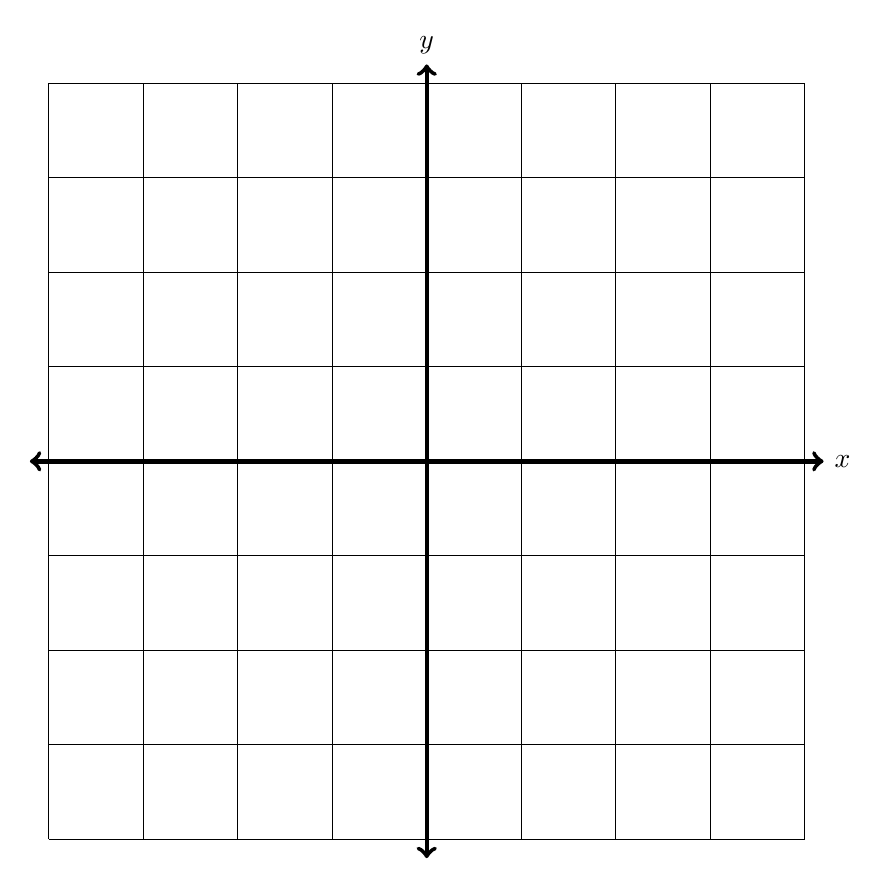
\begin{tikzpicture}[scale = 1.2]
        \draw (-4,-4) grid (4,4);
        \draw[ultra thick, <->] (-4.2,0)--(4.2,0);
        \draw[ultra thick, <->] (0,-4.2)--(0,4.2);
        \node at (4.4,0) {$x$};
        \node at (0,4.4) {$y$};
      \end{tikzpicture}
      \item What is the domain of the function? (i.e. what can go in?)
      \item What is the range of the function? (i.e. what can come out?)
    \end{enumerate}
		\pagebreak
		\item Plot the following functions, and plot at least four points
    (using a calculator to compute decimal approximations if necessary)
    \begin{enumerate}
      \item $g(x) = x^2$ \\
      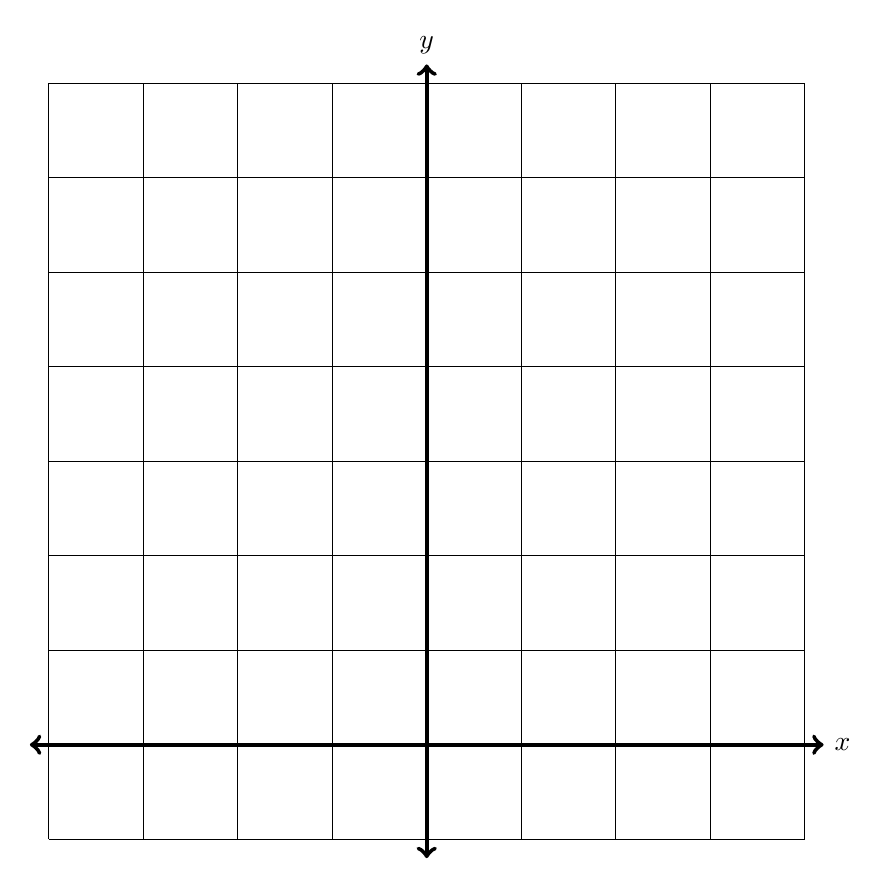
\begin{tikzpicture}[scale = 1.2]
        \draw (-4,-4) grid (4,4);
        \draw[ultra thick, <->] (-4.2,-3)--(4.2,-3);
        \draw[ultra thick, <->] (0,-4.2)--(0,4.2);
        \node at (4.4,-3) {$x$};
        \node at (0,4.4) {$y$};
      \end{tikzpicture}
      \item $g(x) = \sqrt{x}$ \\
      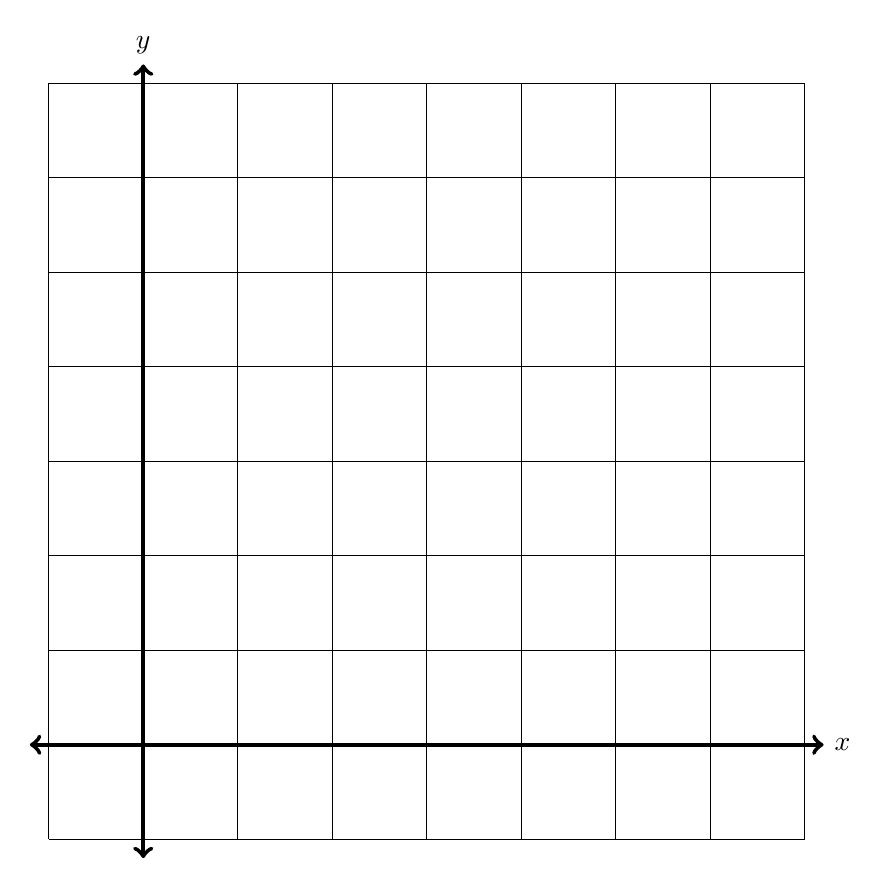
\begin{tikzpicture}[scale = 1.2]
        \draw (-4,-4) grid (4,4);
        \draw[ultra thick, <->] (-4.2,-3)--(4.2,-3);
        \draw[ultra thick, <->] (-3,-4.2)--(-3,4.2);
        \node at (4.4,-3) {$x$};
        \node at (-3,4.4) {$y$};
      \end{tikzpicture}
      \item $h(x) = |x|$ \\
      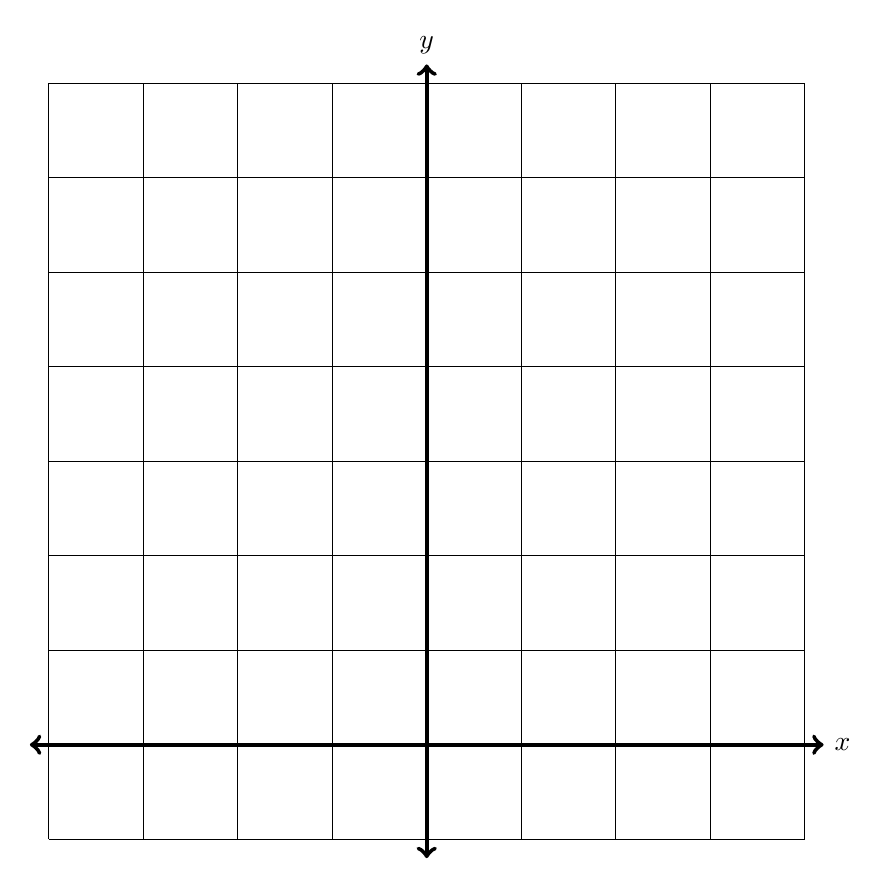
\begin{tikzpicture}[scale = 1.2]
        \draw (-4,-4) grid (4,4);
        \draw[ultra thick, <->] (-4.2,-3)--(4.2,-3);
        \draw[ultra thick, <->] (0,-4.2)--(0,4.2);
        \node at (4.4,-3) {$x$};
        \node at (0,4.4) {$y$};
      \end{tikzpicture}
      \item $F_1(x) = |x|$, $F_2(x) = -|x|$, and $F_3(x) = |x-1|$
      on the same plot. \\
      \textit{Notice that $F_2$ and $F_3$ are shifts of $F_1$.} \\
      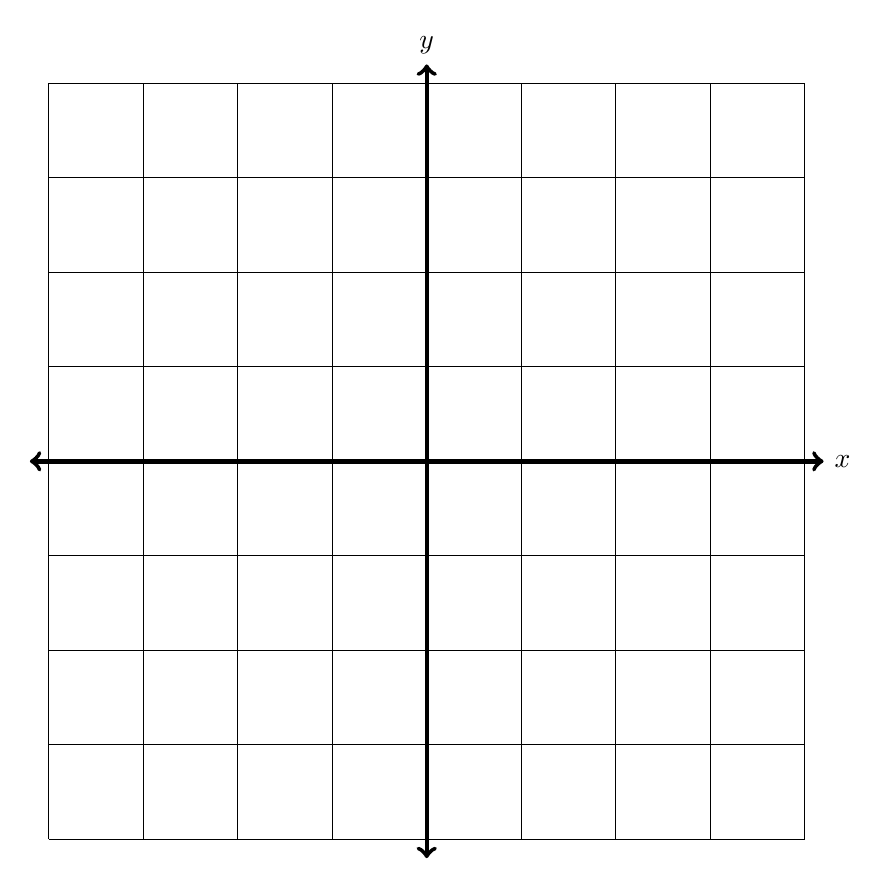
\begin{tikzpicture}[scale = 1.2]
        \draw (-4,-4) grid (4,4);
        \draw[ultra thick, <->] (-4.2,0)--(4.2,0);
        \draw[ultra thick, <->] (0,-4.2)--(0,4.2);
        \node at (4.4,0) {$x$};
        \node at (0,4.4) {$y$};
      \end{tikzpicture}
    \end{enumerate}
    \pagebreak
    \item Graph the following lines. (Solve for $y$ if necessary.)
    \begin{enumerate}
      \item $\displaystyle y - 1 = -\frac 12(x + 2)$ \textit{(point-slope form)}\\
      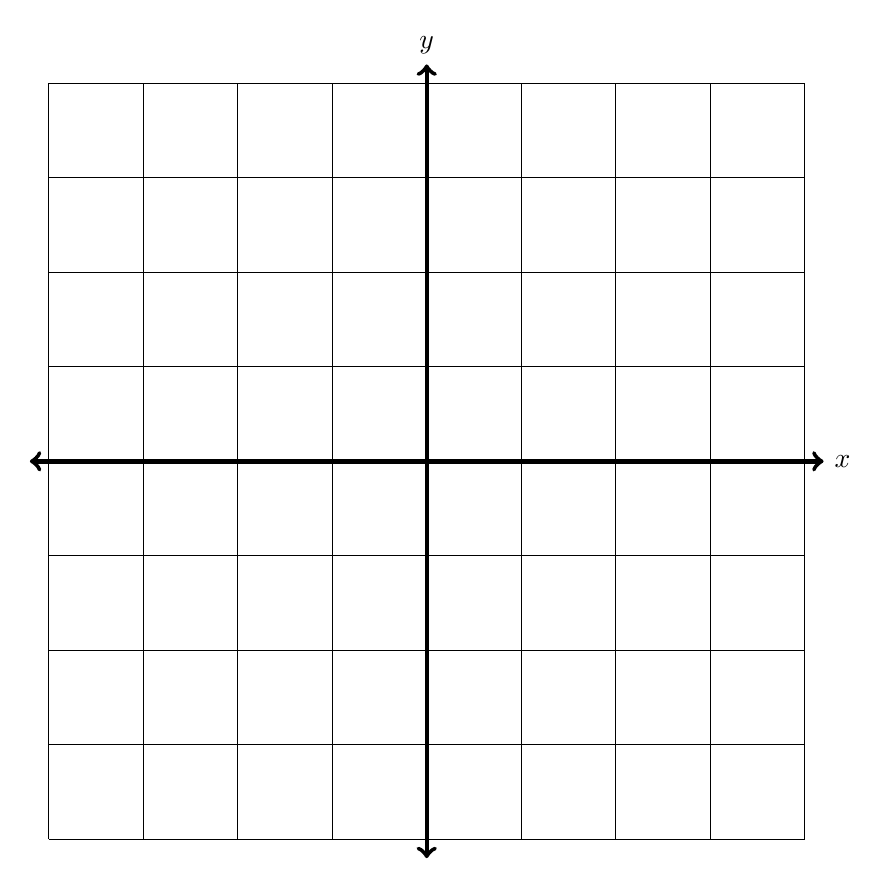
\begin{tikzpicture}[scale = 1.2]
        \draw (-4,-4) grid (4,4);
        \draw[ultra thick, <->] (-4.2,0)--(4.2,0);
        \draw[ultra thick, <->] (0,-4.2)--(0,4.2);
        \node at (4.4,0) {$x$};
        \node at (0,4.4) {$y$};
      \end{tikzpicture}
      \item $3x + 4y = 12$ \textit{(standard form)}\\
      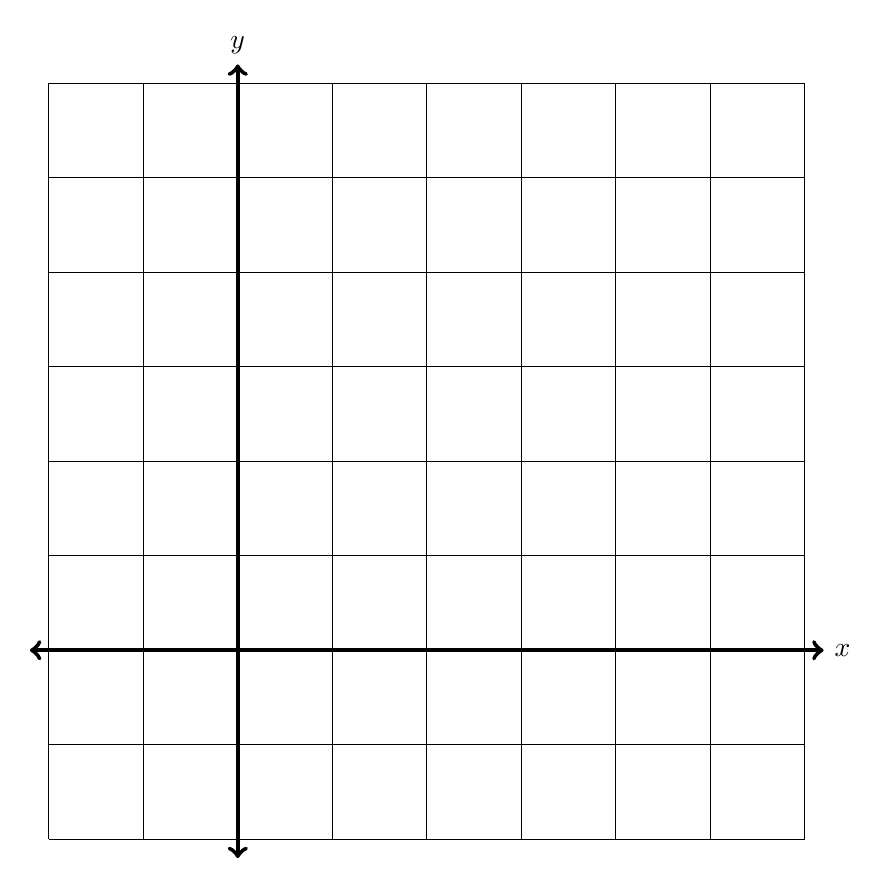
\begin{tikzpicture}[scale = 1.2]
        \draw (-4,-4) grid (4,4);
        \draw[ultra thick, <->] (-4.2,-2)--(4.2,-2);
        \draw[ultra thick, <->] (-2,-4.2)--(-2,4.2);
        \node at (4.4,-2) {$x$};
        \node at (-2,4.4) {$y$};
      \end{tikzpicture}
      \item $y = 2.5$ \textit{(horizontal line)}\\
      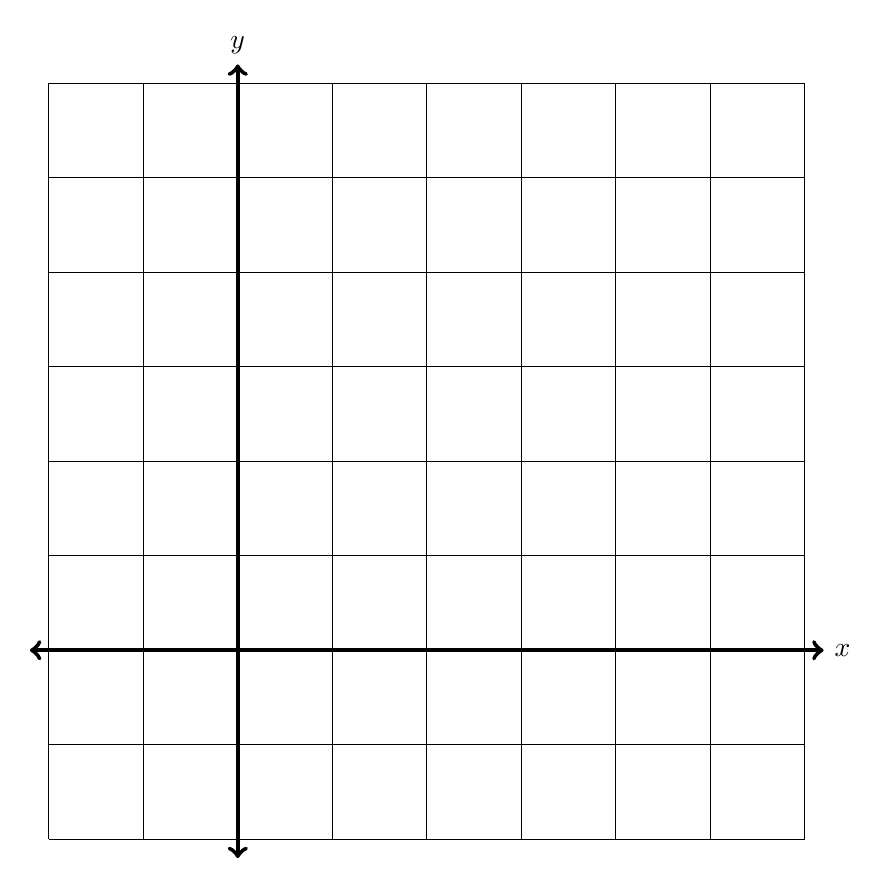
\begin{tikzpicture}[scale = 1.2]
        \draw (-4,-4) grid (4,4);
        \draw[ultra thick, <->] (-4.2,-2)--(4.2,-2);
        \draw[ultra thick, <->] (-2,-4.2)--(-2,4.2);
        \node at (4.4,-2) {$x$};
        \node at (-2,4.4) {$y$};
      \end{tikzpicture}
      \item $y = -\frac 53 x + 4$ \textit{(slope-intercept form)}\\
      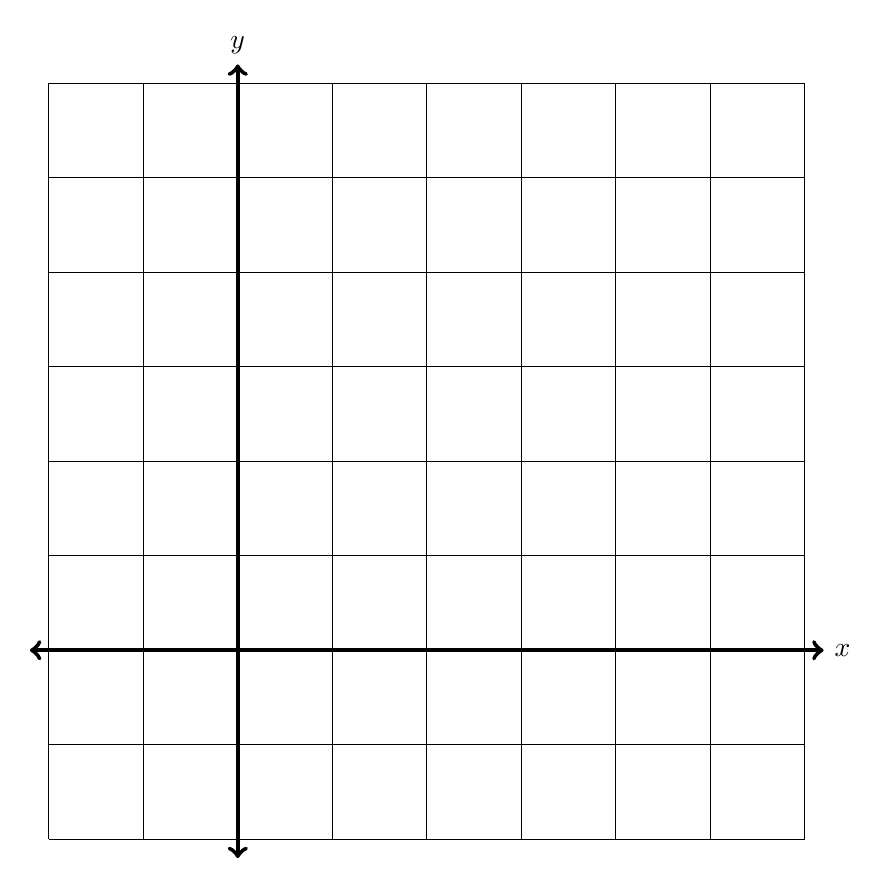
\begin{tikzpicture}[scale = 1.2]
        \draw (-4,-4) grid (4,4);
        \draw[ultra thick, <->] (-4.2,-2)--(4.2,-2);
        \draw[ultra thick, <->] (-2,-4.2)--(-2,4.2);
        \node at (4.4,-2) {$x$};
        \node at (-2,4.4) {$y$};
      \end{tikzpicture}
      \pagebreak
      \item $x = 1.8$ \textit{(vertical line)}\\
      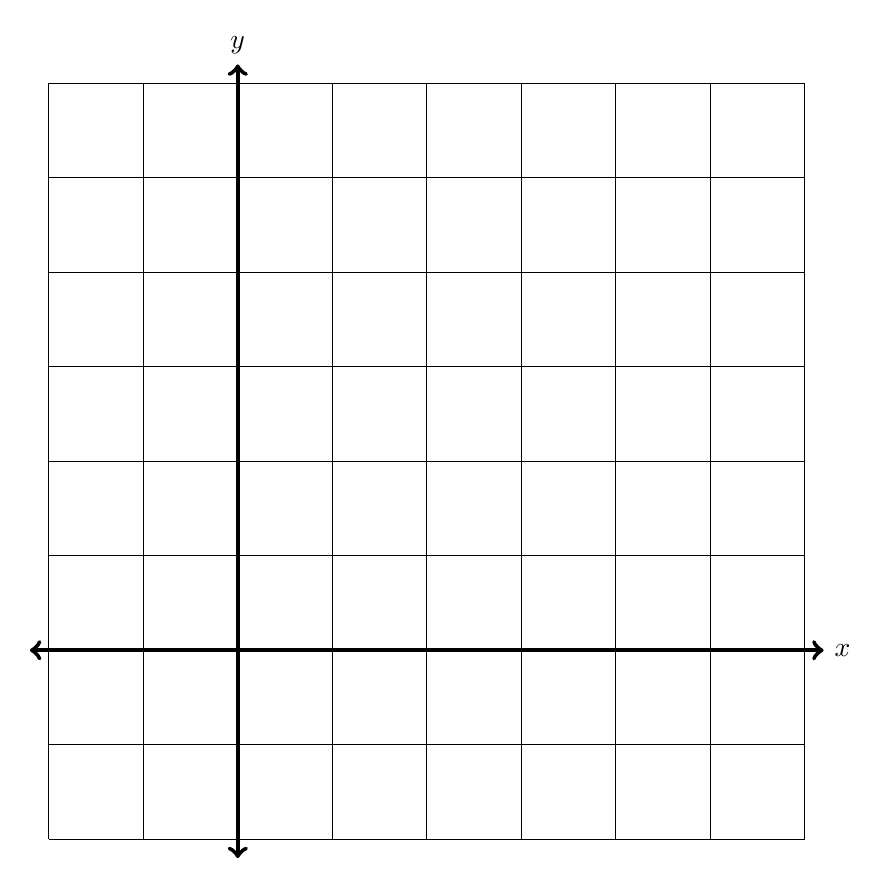
\begin{tikzpicture}[scale = 1.2]
        \draw (-4,-4) grid (4,4);
        \draw[ultra thick, <->] (-4.2,-2)--(4.2,-2);
        \draw[ultra thick, <->] (-2,-4.2)--(-2,4.2);
        \node at (4.4,-2) {$x$};
        \node at (-2,4.4) {$y$};
      \end{tikzpicture}
    \end{enumerate}
    \item In each part, find the equation of the line subject to the following
    conditions
    \begin{enumerate}
      \item The line contains the point $(0, 1)$ and is perpendicular to the
      line $y = \frac 23 x - 100$. \vspace{4cm}
      \item The line crosses the origin and is parallel to the
      line $2y + 6x = 3.5$. \pagebreak
      \item \textit{(Hard)} The line contains the point $(3, 4)$ and is
      perpendicular to the line $\displaystyle y = \frac{9}{19}$.
      \vspace{6cm}
      \item \textit{(Hard)} The line contains the point $(1, -3)$ and is
      perpendicular to the line $x = -7.26$.
      \vspace{6cm}
    \end{enumerate}
    \item Find the range and the domain of the following functions.
    \begin{enumerate}
      \item $f(x) = 2 + \sqrt{x - 1}$
      \textit{(Can you input $0$? $5$? $-5$? Can you get $3$ as an output? $-3$?)}
      \pagebreak
      \item $\displaystyle g(x) = \frac{3}{x^2}$ \\
      \textit{(What can't you divide by? Is it possible to get $0$ as an output? $-1$? $3$?)}
      \vspace{6cm}
      \item $
      \displaystyle h(x) = \begin{cases}
        |x + 1| & -2 \leq x \leq 1 \\
        \sqrt{x - 3} & x > 3
      \end{cases}
      $
      \\
      \textit{(Can you input $-3$? $0$? $1$? $3$?) Can you get a negative output?}
      \vspace{10cm}
      \item $\displaystyle F(x) = -\frac{2}{7}x - \frac{11}{23}$.
    \end{enumerate}
  \end{enumerate}

\end{document}
